%-----------------------------------------------------------------------------------------------%
%
% Maret 2019
% Template Latex untuk Tugas Akhir Program Studi Sistem informasi ini
% dikembangkan oleh Inggih Permana (inggihjava@gmail.com)
%
% Template ini dikembangkan dari template yang dibuat oleh Andreas Febrian (Fasilkom UI 2003).
%
% Orang yang cerdas adalah orang yang paling banyak mengingat kematian.
%
%-----------------------------------------------------------------------------------------------%

%-----------------------------------------------------------------------------%
\chapter{\babDua}
%-----------------------------------------------------------------------------%

%-----------------------------------------------------------------------------%
\section{Penelitian Terdahulu}
%-----------------------------------------------------------------------------%
Beberapa peneliti sebelumnya telah melakukan penelitian tentang kualitas sistem informasi akademik dengan menggunakan metode Mccall dengan kriteria Operasi Produk. Penelitian Andria dkk. (2016) melibatkan pengembang, mahasiswa, dan dosen web portal STT Dharma Iswara Madiun. Hasil penelitian menunjukkan bahwa nilai yang dihasilkan menunjukkan bahwa kualitas web portal STT Dharma Iswara Madiun. Selanjutnya, penelitian Anggraini (2018) melibatkan siswa S1 dari tahun 2013–2016. Hasil penelitian menunjukkan bahwa setiap komponen menunjukkan bahwa website Lembaga Pendidikan Fakultas Ilmu Komputer Uni versitas Brawijaya memiliki kualitas yang sangat baik.Penelitian berikutnya dilakukan oleh Hidayati dkk. (2017), di mana responden adalah mahasiswa Politeknik Negeri Jakarta (PNJ). Hasil penelitian menunjukkan bahwa SIAK PNJ telah memenuhi faktor kualitas perangkat lunak dan kebutuhan mahasiswa PNJ, tetapi masih ada beberapa kekurangan dalam hal keakuratan, efisiensi, dan integritas. 

Penelitian berikutnya adalah  Mandala dan Dewanto (2017), dimana pada penelitian tersebut yang menjadi respondennya adalah siswa SMK Muhamadiyah 1 Bantul. Hasil dari penelitian tersebut adalah uji kelayakan sistem informasi unit kesehatan sekolah berbasis website di SMK 1 Bantul diperoleh hasil kelayakan oleh ahli dari indikator Correctness sebesar 78\%, Reliability sebesar 78\%, Efficiency sebesar 76\%, Integrity 76\%, dan Usability sebesar 81\% dengan kategori layak (Baik) dan dari hasil penilaian kelayakan yang diberikan oleh pengguna dari indikator Correctness sebesar 63,33\%, Reliability 56,66\%, Efficiency sebesar 63,33\%, Integrity sebesar 56,66\% dan Usability sebesar 80\%. Penelitian berikutnya adalah Khairullah dkk. (2017), dimana pada penelitian tersebut yang menjadi respondennya adalah pengguna sistem inventaris aset. Hasil dari penelitian tersebut adalah pengukuran aplikasi sistem inventaris aset mendapatkan nilai dengan persentase 68,4\% dan termasuk dalam kategori baik Dari hasil penilaian oleh pihak praktisi atau pengguna aplikasi tersebut dapat diambil kesimpulan bahwa sistem informasi unit kesehatan sekolah berbasis website di SMK 1 Bantul sangat layak untuk digunakan. Berdasarkan hasil dari beberapa penelitian yang telah dijelaskan sebelumnya, dapat disimpulkan bahwa metode Mccall ini sangat cocok digunakan untuk penelitian kualitas sistem.


% Berikut cara membuat tulisan \textbf{bold}, \textit{italic}, dan \underline{underline} ini dia: 

% \begin{enumerate}
% 	\item \textbf{Bold}: Gunakan perintah \bslash textbf$\lbrace\rbrace$.
% 	\item \textit{Italic}: Gunakan perintah \bslash textit$\lbrace\rbrace$.
% 	\item \underline{Underline}: Gunakan perintah \bslash underline$\lbrace\rbrace$.
% \end{enumerate}

%-----------------------------------------------------------------------------%
\section{Profil Instansi}
%-----------------------------------------------------------------------------%
\subsection{Sejarah}
%-----------------------------------------------------------------------------%
UIN Suska Riau memiliki fasilitas infrastruktur pendukung Tridharma Perguruan Tinggi yang baik, salah satunya adalah laboratorium terpadu di bawah Fakultas Sains dan Teknologi yang dikelola oleh Program Studi Sistem Informasi sejak tahun 2002. Terdapat tiga laboratorium yang dikelola oleh Program Studi Sistem Informasi, yaitu Laboratorium Rekayasa Sistem Informasi (RSI), Laboratorium Internet (INT), dan Laboratorium \textit{Software Engineering} (SE). Ketiga laboratorium tersebut merupakan aset penting yang dapat dimanfaatkan dengan baik untuk mencapai target-target universitas dan menghasilkan lulusan Program Studi Sistem Informasi yang kompeten dalam pendidikan, penelitian, serta pengabdian masyarakat dengan mengintegrasikan nilai-nilai keislaman. Laboratorium-laboratorium tersebut tidak hanya digunakan untuk praktikum mahasiswa sesuai dengan kurikulum, tetapi juga mampu mendukung berbagai kegiatan mahasiswa dan dosen dalam meningkatkan pengetahuan di bidang Sistem Informasi.
% -----------------------------------------------------------------------------%
\subsection{Visi}
% -----------------------------------------------------------------------------%
Menjadi laboratorium Program Studi Sistem Informasi yang memiliki keunggulan dalam bidang pendidikan, penelitian, dan pengabdian kepada masyarakat dengan menghasilkan lulusan yang proaktif, inovatif, dan profesional dalam bidang Sistem Informasi di tingkat lokal, regional, dan nasional yang berbasis nilai-nilai islami pada tahun 2030.
% -----------------------------------------------------------------------------
\subsection{Misi}
% -----------------------------------------------------------------------------%
Untuk mencapai Visi Laboratorium Program Studi Sistem Informasi, berikut Misi-misi yang harus dicapai, diantaranya:

\begin{enumerate}

  \item Mendukung penyelenggaraan kegiatan pendidikan akademik dan praktikum berbasis teknologi kepada mahasiswa, dosen, dan stakeholder.
  \item Mendukung pelaksanaan kegiatan penelitian yang berbasis teknologi kepada mahasiswa, dosen, dan stakeholder.
  \item Mendukung kegiatan pengabdian kepada masyarakat yang berbasis teknologi.
  \item Menyiapkan sumber daya manusia yang mampu menerapkan teknologi informasi khususnya dibidang Sistem Informasi.
  \item Membangun kemitraan dan jejaring dengan industri, pemerintah, dan organisasi nasional.

\end{enumerate}
% -----------------------------------------------------------------------------%
\subsection{Struktur Organisasi}
% -----------------------------------------------------------------------------%
Untuk menjalankan Tridharma Perguruan Tinggi dengan baik, pengelola laboratorium harus memiliki kemampuan manajerial yang baik dan dibantu dengan keahlian IT. Untuk mencapai hal ini, diperlukan sekelompok pengelola laboratorium yang percaya diri dan memiliki kemampuan. Gambar 2.1 menunjukkan struktur organisasi pengelola laboratorium Program Studi Sistem Informasi dari 2021 hingga 2024.

\begin{figure}
  \centering
  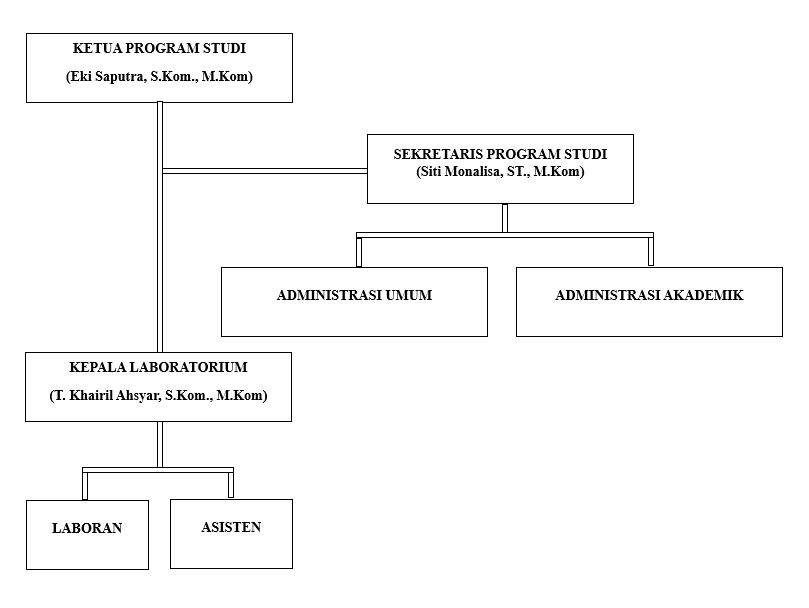
\includegraphics[width=0.82\linewidth]{konten//gambar/Struktur Organisasi.png}
  \caption{Struktur Organisasi Laboratorium}
  \label{fig:enter-label}
\end{figure}

\section{Inventaris}
Inventaris merupakan sebuah kata yang diasimilasikan dari kata \textit{inventory} yang berasal dari bahasa Inggris. Echols dan Shadily merumuskan dalam kamus Besar Bahasa Indonesia sebagai daftar barang disertai dengan nilainya masing-masing yang dimilki perusahaan dalam kurun waktu tertentu yang digunakan dalam kegiatan usaha perusahaan. Dalam praktek, inventaris disebut juga sebagai persediaan barang yang artinya barang-barang biasanya dapat dijumpai digudang tertutup, lapangan, gudang terbuka atau tempat-tempat penyimpanan lain, baik berupa bahan baku, barang setengah jadi, barang jadi barang-barang untuk keperluan operasi atau barang-barang untuk keperluan suatu proyek \cite{novendri2019aplikasi}.
% -----------------------------------------------------------------------------%
\section{Sistem Informasi Inventaris}
% -----------------------------------------------------------------------------%
Sistem informasi adalah suatu sistem didalam Organisasi yang mempertemukan kebutuhan pengolahan transaksi harian, mendukung operasi bersifat manajerial dan kegiatan strategi dari suatu organisasi dan menyediakan pihak luar tertentu dengan laporan-laporan yang diperlukan \cite{laila2011sistem}. Sistem informasi inventaris adalah suatu sistem yang digunakan untuk mengelola dan memantau inventaris atau barang yang dimiliki oleh suatu organisasi atau perusahaan. Sistem ini dapat membantu memudahkan petugas inventaris dalam pendataan barang yang dimiliki oleh organisasi atau perusahaan tersebut \cite{Yanti2021SISTEMII}.
%-----------------------------------------------------------------------------%
%-----------------------------------------------------------------------------%
\section{Laboratorium}
Laboratorium merupakan sarana dalam melaksanakan sebuah riset dalam bidang ilmiah, eksperimen, pengukuran maupun pelatihan ilmiah. Meski laboratorium telah memiliki alat-alat yang lengkap, pengelolaan laboratorium juga harus diperhatikan. Adanya alat-alat yang sudah lengkap dan penggunaan yang sudah baik tentunya perlu untuk dilakukan manajemen yang baik pada laboratorium tersebut, karena terdapat beberapa hal yang harus diperhatikan kembali seperti pengelolaan masing-masing laboratorium dan pengolahan data \cite{sweden2022rancang}.
\subsection{Laboratorium Rekayasa Sistem Informasi (RSI)}
Laboratorium Rekayasa sistem Informasi atau yang disingkat dengan nama Laboratorium RSI merupakan laboratorium pertama yang dimiliki oleh Program Studi Sistem Informasi sejak pindahnya aktivitas perkuliahan kampus dari kampus Sukajadi ke kampus utama Panam Pekanbaru Riau pada tahun 2007. Fungsi utama dari laboratorium ini adalah sebagai fasilitas infrastruktur pendukung untuk pelaksanaan kegiatan perkuliahan praktikum bagi mahasiswa Program Studi Sistem Informasi terkait bidang Rekayasa Sistem Informasi. Bidang Rekayasa Sistem Informasi merupakan bidang yang paling dominan yang ada di Program Studi Sistem Informasi \cite{lab-si-website}.

\subsection{Laboratorium Internet (INT)}
Laboratorium Internet atau yang disingkat dengan nama Laboratorium INT merupakan laboratorium milik Program Studi Sistem Informasi di bawah Fakultas Sains dan Teknologi kedua yang aktivitas perkuliahannya berada di kampus utama Panam Pekanbaru Riau. Secara spesifik, laboratorium ini lebih dioperasikan untuk kebutuhan perkuliahan terkait matakuliah praktikum dasar, seperti matakuliah Jaringan Komputer dan Pemrograman Dasar \cite{lab-si-website}.

\subsection{Laboratorium \textit{Software Engineering} (SE)}
Laboratorium ke tiga yang dimiliki oleh Program Studi Sistem Informasi adalah Laboratorium \textit{Software Engineering} atau yang disingkat dengan nama Laboratorium SE. Laboratorium ini merupakan laboratorium terbaru milik yang dikelola oleh Program Studi dari usulan pengadaan barang tahun anggaran 2021 di bawah naungan Fakultas Sains dan Teknologi UIN Suska Riau. Adapun laboratorium SE sebagai pendukung dalam pelaksanaan kegiatan perkuliahan praktikum bagi mahasiswa Program Studi Sistem Informasi yang terkait dengan bidang keilmuan seperti Praktikum Basis Data, Pemrograman Beorientasi Objek (PBO), dan matakuliah wajib praktikum lainnya \cite{lab-si-website}.

\section{SITARIS SI}

\section{Evaluasi}
Evaluasi merupakan bagian yang sangat penting dalam sebuah organisasi untuk penilaian. Evaluasi dapat diartikan sebagai proses pengukuran akan efektiv itas startegi yang digunakan dalam upaya mencapai tujuan organisasi (Al Agani, Munadi, dan Subianto, 2018). Adapun tujuan dan fungsi dari evaluasi yaitu, un tuk mengetahui apakah tujuan-tujuan yang telah ditetapkan telah tercapai dalam kegiatan, untuk memberikan objektivitas pengamatan terhadap perilaku hasil, un tuk mengetahui kemampuan dan menentukan kelayakan, dan untuk memberikan umpan balik bagi kegiatan yang dilakukan. Menurut Adiati (2015) evaluasi dilakukan sebagai uji coba untuk melihat sejauh apa sebuah software dapat dikatakan berkualitas dan sebagai acuan untuk melakukan pengembangan software. Perlunya dilakukan evaluasi agar dapat men gukur fungsionalitas dari portal akademik. Hasil dari evaluasi dapat menyimpulkan 20 fungsi/proses apa yang sudah berjalan dengan baik dan yang belum/tidak berjalan dengan baik (Terttiaavini, 2014).

\subsection{Prosedur Evaluasi}
Menurut Umar (2002) proses suatu evaluasi pada umumnya memilik i tahapan-tahapannya sendiri. Walaupun tidak selalu sama, tetapi yang lebih penting adalah bahwa prosesnya sejalan dengan fungsi evaluasi itu sendiri. Berikut ini di paparkan salah satu tahapan evaluasi yang sifatnya umum digunakan. 1. Menentukan apa yang akan dievaluasi. Dalam bisnis, apa saja yang dapat dievaluasi, dapat mengacu pada program kerja perusahaan. Di sana banyak terdapat aspek-aspek yang kiranya dapat dan perlu dievaluasi. Tetapi, biasanya diprioritaskan untuk dievaluasi adalah hal-hal yang menjadi key-success factors-nya. 2. Merancang (desain) kegiatan evaluasi. Sebelum evaluasi dilakukan, tentukan terlebih dahulu desain evaluasinya agar data apa saja yang dibutuhkan, tahapan-tahapan kerja apa saja yang dilalui, siapa saja yang aka dilibatkan, serta apa saja yang akan dihasilkan menjadi jelas. 3. Pengumpulan data. Berdasarkan desain yang telah disiapkan, pengumpulan data dapat di lakukan secara efektif dan efisien, yaitu sesuai dengan kaidah-kaidah ilmiah yang berlaku dan sesuai dengan kebutuhan dan kemampuan. 4. Pengolahan dan analisis data. Setelah data terkumpul, data tersebut diolah untuk dikelompokkan agar mu dah dianalisis dengan menggunakan alat-alat analisis yang sesuai, sehingga dapat menghasilkan fakta yang dapat dipercaya. Selanjutnya, dibandingkan antara fakta dan harapan atau rencana untuk menghasilkan gap. Besar gap akan disesuaikan dengan tolok ukur tertentu sebagai hasil evaluasinya. 5. Pelaporan hasil evaluasi. Agar hasil evaluasi dapat dimanfaatkan bagi pihak-pihak yang berkepentin gan, hendaknya hasil evaluasi didokumentasikan secara tertulis dan diinfor masikan baik secara lisan maupun tulisan. 6. Tindak lanjut hasil evaluasi. Evaluasi merupakan salah satu bagian dari fungsi manajemen. Oleh karena itu, hasil evaluasi hendaknya dimanfaatkan oleh manajemen untuk mengam bil keputusan dalam rangka mengatasi masalah manajemen, baik ditingkat strategi maupun di tingkat implementasi strategi. 21

\subsection{Standar Evaluasi}
Menurut Umar (2002) standar yang dipakai untuk mengevaluasi suatu kegiatan tertentu dapat dilihat dari tiga aspek utama, yang menurut Committee on Standard for Educational Evaluation kiranya dapat digunakan pula aspek bisnis, yaitu: 1. Manfaat (Utility). Hasil evaluasi hendaknya bermanfaat bagi manajemen untuk pengambilan keputusan atas program yang sedang berjalan. Misal nya, dilakukan evaluasi terhadap bagian dari suatu program promosi yang sedang berjalan, ternyata informasi dari evaluasi kurang bermanfaat dalam pengambilan keputusan, maka hasil evaluasi dianggap tidak bermanfaat. 2. Akurat(Accuracy). Informasiatashasil evaluasi hendaklah memiliki tingkat ketepatan tinggi. Misalnya, dalam program promosi telah disepakati bahwa anggaran promosi sampai tengah tahun akan habis X rupiah dan kegiatan kegiatan yang harus diselesaikan sebanyak Y kegiatan. Setelah dilakukan evaluasi, hendaknya informasinya dapat dipakai untuk menilai apakah real isasi promosi dianggap menyimpang atau tidak. 3. Layak(Feasibility). Hendaknya proses evaluasi yang dirancang dapat dilak sanakan secara layak. Untuk evaluasi program promosi, hendaknya evalu ator dapat melaksanakannya dengan baik dan benar, tidak hanya dari aspek teknis, tetapi juga dari aspek lain, seperti legal dan etis. Suatu evaluasi yang dapat mencapai standar di atas adalah evaluasi yang sifatnya ideal, artinya tidak mudah untuk dilaksanakan. Cronbach dkk. (1980) men gatakan bahwa standar yang digunakan untuk melakukan evaluasi mungkin tidak sepenting konsekuensinya, yaitu bahwa evaluasi yang baik adalah evaluasi yang memberikan dampak positif pada perkembangan pelaksanaan suatu program.

\section{Kualitas Sistem}
Kotler dan Keller mendefinisikan kualitas sebagai keseluruhan fitur dan karakteristik produk atau jasa yang bergantung pada kemampuannya untuk memberikan kepuasan. Sementara itu, Andria, Kusrini, dan Armadyah (2020) me nyatakan bahwa pada tingkat yang lebih praktis, kualitas merupakan konsep yang rumit dan memiliki berbagai aspek yang beragam. Kualitas sistem merujuk pada evaluasi proses sistem informasi dengan fokus pada hasil interaksi antara pengguna dan sistem. Kualitas sistem mencakup atribut atribut seperti ketersediaan peralatan, keandalan peralatan, kemudahan penggunaan, dan waktu respon, yang merupakan faktor-faktor kunci yang mempengaruhi apakah sebuah sistem informasi akan digunakan atau tidak (Pawirosumarto, 2016)

\section{Model McCall}
Pada tahun 1977, Jim McCall dan timnya mengusulkan suatu kerangka penggolongan yang melibatkan faktor-faktor atau kriteria yang memengaruhi pertimbangan kualitas perangkat lunak. McCall berusaha menyatukan perspektif pengguna dan prioritas pengembang yang berfokus pada beberapa faktor kualitas perangkat lunak. Tujuannya adalah untuk meningkatkan mutu produk perangkat lunak (McCall, 1977).

Model yang dikemukakan oleh McCall adalah salah satu model yang menjelaskan Faktor Kualitas Perangkat Lunak atau Software Quality Factor 12 McCall mengintegrasikan tiga perspektif utama dalam kerangka kerjanya, yaitu: 
\begin{enumerate}
	\item \textit{Product Operation}, fokus pada sifat-sifat operasional dari perangkat lunak, yang mencakup aspek-aspek seperti kinerja, kehandalan, efisiensi, dan keamanan dalam penggunaan sehari-hari. 
	\item \textit{Product Revision}, mengukurkemampuanperangkatlunakuntukberadaptasi dan menjalani perubahan. Ini melibatkan faktor-faktor seperti kemudahan pemeliharaan, kegunaan dalam melakukan pembaruan, dan skalabilitas. 
	\item \textit{Product Transition}, mengacu pada kemampuan perangkat lunak untuk beradaptasi dengan lingkungan baru atau berpindah ke platform atau infrastruktur yang berbeda. Ini mencakup fleksibilitas dalam migrasi dan integrasi dengan sistem yang ada.
\end{enumerate}

Dengan mempertimbangkan tiga perspektif ini, McCall berusaha memahami dan mengukur kualitas perangkat lunak dari berbagai sudut pandang yang penting. Pendekatan ini membantu dalam pengembangan perangkat lunak yang lebih berkualitas dan mampu memenuhi kebutuhan pengguna sambil tetap mudah dikelola dan disesuaikan dengan perubahan lingkungan, Model McCall bisa dilihat pada Gambar 2.2 berikut: 

\begin{figure}
  \centering
  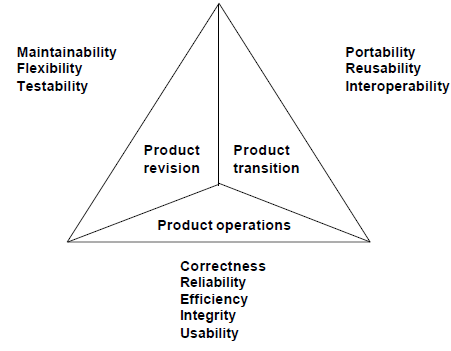
\includegraphics[width=0.82\linewidth]{konten//gambar/Metode McCall.png}
  \caption{Metode McCall}
  \label{fig:enter-label}
\end{figure}

Model McCall dikenal sebagai model yang komprehensif dalam menggambarkan faktor-faktor atau kriteria kualitas perangkat lunak. Kelebihan dari model ini adalah ketelitiannya dan detail yang cermat, sehingga sangat pas untuk pengujian dan memverifikasi kualitas perangkat lunak dalam sistem informasi. 

Dalam Model McCall, ada tiga jenis ciri khas utama kualitas perangkat lunak, yaitu Product Operation, Product Revision, dan Product Transition. Dari 13 ketiga karakteristik ini, penelitian yang dilakukan fokus pada aspek Product Op eration, yang mencerminkan pandangan eksternal perangkat lunak dari pandan gan pengguna (Saputera, Sunardi, Syafrizal, dan Samsidi, 2020). Ini mencakup 12 faktor kualitas yang dijelaskan sebagai berikut: 

\begin{enumerate}
	\item Correctness: Sejauh mana program menepati persyaratan dan mencapai tujuan yang ditetapkan oleh program tersebut. 
	\begin{enumerate}[label=(\alph*)]
		\item Completeness: Faktor ini mengukur sejauh mana implementasi fungsi fungsi yang diinginkan dalam aplikasi dapat dicapai. Dalam kon teks ini, kelengkapan mengacu pada apakah semua fitur dan fungsi yang diharapkan oleh pengguna telah diimplementasikan dengan be nar dalam perangkat lunak. 
		\item Consistency: Konsistensi adalah aspek yang sangat penting dalam desain antarmuka pengguna (UI) dan pengalaman pengguna secara umum. Ini menekankan kesesuaian desain antarmuka pada seti ap tampilan atau halaman dalam aplikasi. Konsistensi memastikan bahwa elemen-elemen UI, tata letak, warna, ikon, dan gaya desain secara keseluruhan seragam dan mudah dipahami oleh pengguna. Konsistensi membantu pengguna merasa nyaman dan tidak bingung saat menggunakan aplikasi. 
		\item Traceability: Kemudahan pelacakan merujuk pada seberapa mu dah pengguna dapat melacak atau mengikuti implementasi atau komponen-komponen perangkat lunak dalam aplikasi. Ini berguna ketika pengguna ingin memahami bagaimana suatu fungsi atau fitur tertentu diimplementasikan dalam perangkat lunak. Dengan adanya kemudahan pelacakan, pengguna dapat dengan cepat menemukan informasi yang mereka cari terkait dengan perangkat lunak. 
\end{enumerate}
	\item Reliability: Sejauh mana program mampu menjalankan fungsi yang dituju dengan tingkat presisi yang sesuai. 
		\begin{enumerate}[label=(\alph*)]
				\item Error Tolerance: Faktor ini mengukur sejauh mana perangkat lunak dapat menangani atau mengatasi kesalahan yang terjadi selama penggunaan. 
				\item Accuracy: Ketepatan adalah faktor yang mengukur sejauh mana perangkat lunak dapat memberikan hasil yang tepat dan akurat dalam pelaksanaan fungsi-fungsi komputasi dan kontrol.
				\item Simplicity: Kesederhanaan mengacu pada tingkat dimana aplikasi atau perangkat lunak dapat dipahami dengan mudah tanpa menyebabkan kesulitan bagi pengguna. Aplikasi yang sederhana memiliki tata letak 14 yang intuitif, navigasi yang jelas, dan instruksi yang mudah dipahami. 
		\end{enumerate}
		
	\item Efficiency: Jumlah sumber daya komputasi yang diperlukan oleh program untuk menjalankan fungsi dengan eksekusi yang efisien. 
	\begin{enumerate}[label=(\alph*)]
		\item Execution Efficiency: Efisiensi eksekusi mengukur sejauh mana perangkat lunak dapat menjalankan tugas atau fungsi dengan menggunakan sumber daya komputasi (seperti CPU, memori, dan jaringan) dengan efisien. Ini berarti perangkat lunak harus dapat melakukan tugasnya dengan seefisien mungkin tanpa memboroskan sumber daya yang tersedia. Efisiensi eksekusi penting karena pengguna ingin aplikasi yang berjalan dengan cepat dan tanpa lag. 
		\item Conciseness: Keringkasan merujuk pada sejauh mana perangkat lunak memiliki kode atau implementasi yang sederhana, ringkas, dan tidak mengandung elemen yang tidak perlu. Semakin konsis dan ringkas perangkat lunak, semakin mudah untuk memahami, mengelo la, dan memelihara. Keringkasan juga dapat meminimalkan peluang kesalahan atau bug dalam kode. 
\end{enumerate}
	\item Integrity: Sejauh mana sistem mampu mencegah akses oleh individu yang tidak memiliki izin. 
	\begin{enumerate}[label=(\alph*)]
		\item Access Control: Kendali akses adalah faktor yang mengukur kemampuan perangkat lunak untuk mengendalikan hak akses pengguna terhadap berbagai modul atau komponen perangkat lunak. 
\end{enumerate}
	\item Usability: Usaha yang dibutuhkan oleh pengguna untuk mempelajari, mengoperasikan, dan memahami hasil dari program. 
	\begin{enumerate}[label=(\alph*)]
		\item Operability: Kemudahan pengoperasian merujuk pada tingkat kenyamanan dan kemudahan dalam menggunakan aplikasi. Faktor ini mencakup sejauh mana pengguna dapat dengan cepat memahami antarmuka dan fungsi aplikasi, serta seberapa mudah mereka dapat menjalankan tugas-tugas yang diinginkan. Aplikasi yang memiliki tingkat kemudahan pengoperasian yang tinggi akan lebih disukai oleh pengguna. 
		\item Training: Faktor pelatihan menilai sejauh mana pengguna memer lukan pelatihan tambahan atau bantuan untuk menggunakan aplikasi. Aplikasi yang mudah dipelajari dan digunakan oleh pengguna tanpa perlu pelatihan yang intens akan memiliki nilai tinggi dalam faktor ini. 
		\item Communicativeness: Kemampuan berkomunikasi mencakup sejauh mana aplikasi dapat menyediakan informasi yang transparan dan mudah dimengerti bagi pengguna. Ini termasuk dalam penyampaian pesan atau petunjuk kepada pengguna dalam bentuk yang tidak membin gungkan. Aplikasi yang komunikatif akan membantu pengguna dalam memahami apa yang sebenarnya terjadi dan bagaimana cara berinter aksi dengan aplikasi tersebut. 
\end{enumerate}
\end{enumerate}
Semua faktor-faktor ini memainkan peran penting dalam menentukan kualitas perangkat lunak dan pengalaman pengguna. Dengan memahami dan mengukur faktor-faktor ini, pengembang perangkat lunak dapat memastikan bahwa produk mereka memenuhi standar kualitas yang diharapkan oleh pengguna.

\section{Skala Likert}
Skala Likert memiliki fungsi untuk mengukur sikap, pendapat, dan persep si seseorang atau sekelompok orang tentang fenomena sosial. Dalam penelitian, fenomena sosial ini telah ditetapkan secara spesifik oleh peneliti, yang selanjut nya disebut sebagai variabel penelitian. Dengan Skala Likert, maka variabel yang akan diukur dijabarkan menjadi indikator variabel. Kemudian indikator tersebut di jadikan sebagai titik tolak untuk menyusun item-item instrumen yang dapat berupa pernyataan atau pertanyaan, baik bersifat favorable (positif) bersifat bersifat unfa vorable (negatif) (Fendya dan Wibawa, 2018). Skala likert digunakan untuk mendapatkan data pada uji validitas perangkat lunak. Peneliti telah menyediakan empat alternatif jawaban, yaitu: Sangat Setuju (SS) = 4 Setuju(S) = 3 Tidak Setuju(TS) = 2 Sangat Tidak Setuju (STS) = 1

\section{Observasi}
Observasi adalah tindakan mengamati secara langsung perilaku individu, objek, atau aktivitas dengan cara yang teratur tanpa melakukan interaksi lansung dengan subjek yang diamati (Sangadji, 2010). Observasi merupakan metode pengumpulan data di mana pengamat mengamati suatu sistem atau entitas saat sedang beroperasi untuk mendapatkan wawasan dan pemahaman yang lebih mendalam tentang bagaimana sistem tersebut bekerja (Tilley dan Rosenblatt, 2017).

\section{Populasi dan Sampel}
\subsection{Populasi}
Menurut Sedarmayanti dan Hidayat (2011), populasi ialah kumpulan seluruh ciri-ciri yang mendefinisikan objek penelitian. Definisi lain mengenai populasi adalah seluruh subjek psikologis yang memenuhi persyaratan tertentu. Terkait dengan objek yang termasuk dalam populasi, ada dua jenis dimensi populasi yang diakui: 1. Populasi Tak Hingga adalah populasi yang memiliki jumlah objek yang tak terbatas. Contoh dari jenis populasi ini adalah semua pengamatan tentang proses yang berlangsung secara terus-menerus di bawah kondisi yang sama. 2. Populasi Terhingga adalah semua populasi yang memiliki jumlah objek 17 yang terbatas.
\subsection{Sampel}
Sedarmayanti dan Hidayat (2011) juga mengatakan bahwa sampel ialah bagian kecil yang diperhatikan dan mewakili karakteristik populasi, sehingga ciri dan atribut yang ada pada populasi juga hadir dalam sampel tersebut. Dalam pene litian ini, digunakan Teknik Sampling Purposive. Teknik Sampling Purposive adalah metode penentuan sampel yang didasarkan pada pertimbangan peneliti atau evaluator mengenai sampel mana yang paling bermanfaat dan representatif. Terkadang, penentuan sampel dilakukan berdasarkan pengetahuan tentang suatu populasi, anggota-anggotanya, dan tujuan penelitian. Pendekatan ini sangat efektif digunakan dalam studi penjajagan, yaitu studi awal untuk penelitian atau evaluasi, yang kemudian dapat diikuti oleh pene litian lebih lanjut dengan pengambilan sampel secara acak (random) (Retnawati, 2017). Dalam upaya pengambilan sampel yang diperlukan, penulis memanfaatkan metode Slovin untuk menghitung jumlah sampel minimal yang diperlukan ketika ukuran populasi telah diketahui. Persamaan 2.1 adalah Rumus Slovin: n = N 1+Ne2 Keterangan: N=jumlah populasi n =jumlah sampel e =nilai presisi (tingkat kepercayaan 90\% maka e = 10\%) (Azrullah, 2021)
\subsection{Prosedur Probabilitas Sampling}
Prosedur sampling probabilitas menjelaskan bahwa peneliti memilih atau mengambil sampel dari suatu populasi yang diketahui informasinya, yaitu sampling frame. Pemilihan sampel acak memberi kesempatan yang sama kepada seluruh unit dalam suatu populasi terpilih sebagai sampel penelitian. Keunggulan utama teknik sampling acak adalah akurasi dan presisi dapat dicapai sehingga hasil penelitian da pat digeneralisasi. Berikut adalah teknik-teknik dalam proses sampling probabilitas menurut Boediono (2001). 1. Sampling acak sederhana (simple random sampling) Teknik sampling acak sederhana efektif dan efisien digunakan pada populasi yang bersifat homogen. 2. Sampling acak sistematik (systematic random sampling) Sampling acak sistematik merupakan pemilihan sejumlah sampel dari suatu populasi secara acak namun sistematis. 3. Sampling acak berstrata (stratified random sampling) Sampling acak berstrata merupakan pemilihan sejumlah sampel dari suatu populasi secara acak dan berdasar pada strata tertentu. Seperti pada pemili han sampel acak sederhana yang sistematik. 4. Sampling kluster (cluster sampling) Teknik sampling kluster merupakan pemilihan sejumlah sampel dari suatu populasi secara acak pada suatu kluster tertentu. Seperti pada pemilihan sampel acak sederhana dan sistematik, peneliti memiliki data tentang pop ulasi berupa sampling frame. Peneliti kemudian menggunakan daftar pop ulasi tersebut untuk menentukan kluster dan memilih sampel secara acak dalam tiap kluster. 5. Sampling ganda (double sampling) Sampling ganda sedikit berbeda dengan 4 teknik sampling acak sebelum nya. Sampling ganda merupakan kombinasi dua atau tiga teknik tersebut. Teknik sampling ini digunakan untuk mendapatkan sinergi keunggulan dari tiga teknik sampling di atas. Pada prinsipnya, peneliti tetap memiliki data tentang populasi berupa sampling frame. Peneliti kemudian memilih sampel secara acak dengan mengombinasikan dua atau tiga teknik sampling acak di atas
\subsection{Prosedur Probabilitas Non Sampling}
Prosedur sampling non probabilitas adalah memilih atau mengambil sampel dari suatu populasi yang tidak diketahui informasinya, yaitu tanpa sampling frame. Pemilihan sampel non probabilitas tidak memberi kesempatan yang sama kepada seluruh unit atau entitas dalam suatu populasi terpilih sebagai sampel penelitian. Kelemahan utama prosedur sampling non probabilitas adalah presisi dan akurasi yang sulit dicapai sehingga hasil penelitian tidak dapat digeneralisasi berikut adalah teknik-teknik dalam prosedur non probabilitas. 1. Sampling mudah (convenience sampling) Teknik sampling mudah merupakan teknik pemilihan sampel ketika peneli ti tidak memiliki data tentang populasi dalam bentuk sampling frame dan peneliti kemudian memilih sampel berdasarkan prinsip kemudahan dalam mengambil atau memilih sampel. 2. Sampling bertujuan (purposive sampling) Teknik sampling bertujuan merupakan teknik pemilihan sampel ketika peneliti tidak memiliki data tentang populasi dalam bentuk sampling frame dan peneliti kemudian memilih sampel berdasarkan kriteria-kriteria terten tu dan penilaian peneliti untuk mengarahkan sampel terpilih sesuai dengan tujuan penelitian. 3. Sampling bergulir (snowball sampling) Teknik sampling bergulir merupakan teknik pemilihan sampel ketika peneli ti tidak memiliki data tentang populasi dalam bentuk sampling frame dan peneliti kesulitan menemukan sampel secara langsung. Teknik ini berbeda dengan teknik sampling lainnya karena situasi khusus dan konteks peneli tian khusus sehingga peneliti membutuhkan cara khusus pula untuk mem peroleh data dari sampel penelitian. Teknik ini umumnya digunakan oleh studi-studi kualitatif dan studi sains kritis
\section{SPSS}
Menurut (Adiati, 2015) Statistical Package for the Social Sciences (SPSS)
adalah salah satu aplikasi yang sering digunakan dalam mengolah dan menganalisis
data statistik. Pada penelitian ini, SPSS akan digunakan untuk mengolah data kue
sioner mengenai kualitas sistem dan selanjutnya akan dilakukan uji reliabilitas dan
validitas sehingga mendapatkan data yang paling reliabel dan valid.
